\documentclass[conference]{IEEEtran}
\makeatletter
\def\ps@headings{%
\def\@oddhead{\mbox{}\scriptsize\rightmark \hfil \thepage}%
\def\@evenhead{\scriptsize\thepage \hfil \leftmark\mbox{}}%
\def\@oddfoot{}%
\def\@evenfoot{}}
\makeatother
\pagestyle{headings}

\IEEEoverridecommandlockouts
 \usepackage{array}
% \usepackage{algorithm2e}
% \usepackage{algorithmicx}
% \usepackage{algorithm}% http://ctan.org/pkg/algorithms
% \usepackage{algpseudocode}% http://ctan.org/pkg/algorithmicx
\usepackage{cite}

\newtheorem{mydef}{Definition}

% *** GRAPHICS RELATED PACKAGES ***
%
\ifCLASSINFOpdf
  \usepackage[pdftex]{graphicx}
\else
  \usepackage[dvips]{graphicx}
\fi


\usepackage{float}

% *** MATH PACKAGES ***
%

\usepackage{xfrac}
%\usepackage{algorithmicx}
\usepackage{algorithm}% http://ctan.org/pkg/algorithms
\usepackage{algpseudocode}% http://ctan.org/pkg/algorithmicx





\usepackage[cmex10]{amsmath}
\usepackage{amssymb}
\usepackage{xfrac}
\usepackage{xfrac}
\usepackage{color}
\usepackage[normalem]{ulem} 
\newcommand{\schange}[2]{ \sout{#1} {\color{green} #2 }}
\newcommand{\question}[1]{ {\color{red} #1 }}
\newtheorem{theorem}{Theorem}[section]
\newtheorem{lemma}[theorem]{Lemma}
\usepackage[caption=false,font=footnotesize]{subfig}
\usepackage{url}
% \usepackage{hyperref}
\hyphenation{op-tical net-works semi-conduc-tor}

\newcommand*{\PROB}{\mathbf{P}}

%%versions
% \usepackage{versions}
% \includeversion{conf}
% \excludeversion{extended}

%  \includeversion{extended}
%  \excludeversion{conf}


\begin{document}
\title{Detection Mechanism for Internal Attacks on Pull-based P2P Video Streaming Systems}

% \author{\IEEEauthorblockN{Hatem Ismail}
% \IEEEauthorblockA{DEEDS Group, TU Darmstadt\\
% % Darmstadt, Germany\\
% hayman@deeds.informatik.tu-darmstadt.de}
% \and
% \IEEEauthorblockN{Stefanie Roos}
% \IEEEauthorblockA{University of Waterloo \\
% % Waterloo, Canada\\
% stefanie.roos@uwaterloo.ca}
% \and
% \IEEEauthorblockN{Giang Nguyen}
% \IEEEauthorblockA{TU Dresden\\
% % Darmstadt, Germany\\
% giang.nguyen@tu-dresden.de}
% \and
% \IEEEauthorblockN{Neeraj Suri}
% \IEEEauthorblockA{DEEDS Group, TU Darmstadt\\
% % Darmstadt, Germany\\
% suri@cs.tu-darmstadt.de}
% }


% make the title area
\maketitle

\begin{abstract}

Online streaming is a very popular service and P2P-based solutions for streaming can reduce costs for both providers and users.
Yet, involving users into the data dissemination entails security risks including a variety of denial-of-service attacks. 
While extensive research exists on mitigating varied attack types, the class of inference attacks (where the attacker is capable of inferring the peers directly connected to the source), still constitutes a major open threat for streaming P2P systems.

Our research focuses on the critical class internal inference attacks for pull-based overlays, where the attacker first infers the overlay's topology before conducting a buffer-map ($BM$) cheating attack using malicious peers located at the positions closest to the source. 
We demonstrate the feasibility of conducting such attacks, and also show how very few malicious peers can drastically compromise the P2P overlay.

Accordingly, we propose a two-fold detection mechanism that is capable of (a) detecting the malicious peers conducting dropping $BM$ cheating behavior in the worst case scenario where 100\% of the sources neighbors are malicious, and (b) restoring the the overlay to a benign state.
The proposed mechanism allows peers to collaboratively detect and notify the source, which in turn replaces the suspected peers.

Using a combined theoretical and simulation-based analysis, we validate that the detection mechanism is able to detect malicious peers with up to 80-90\% accuracy while inducing a small overhead of approximately 8\%. Furthermore, we ascertain theoretically and through simulations that malicious peers cannot misuse the detection mechanism to gain influence. 
% \mn[Stef]{What is a `benign state'? sounds like we actually remove nodes} 
% \mn[Stef]{detecting the worst-case attack is not really an achievement, detecting less obvious attacks is... I would rewrite this}
% Simultaneously, peers locally sanitize their contact lists from peers who conduct adversarial $BM$ cheating behaviors.



\end{abstract} 
\section{Introduction}
\label{sec:intro}

Over the last few years, the attraction, and thus reliance, on streaming P2P systems is continuously growing. 
Accordingly, a remarkable number of P2P streaming applications are available in the market with a very close competition to gain users trust.
As users are mainly oriented about safety and QoS when selecting an application, a lot of research has been conducted that focuses on these particular issues.

In this context, several data dissemination techniques that target optimizing the user's experience in terms of the utilizing the upload and download bandwidth.
With outperforming other dissemination techniques, \textit{pull-based} is the most popular/convenient approach used in most of the existing applications [ref1,ref2].
In a pull-based streaming system, peers actively advertise and request video chunks through a periodic exchange of their buffer-maps in a mesh overlay.

In fact, authenticating, tracking or monitoring operations in a pull-based system is very challenging due to the tight constraints of a distributed online stream, where peers posses limited bandwidth, resources and in-tolerable delay constraints [ref3, ref4, ref5].
Moreover, in [ref6, SWAP, RBCS], the authors pointed out to the possibility of inferring the overlay structure and thus, sabotaging the system by externally attacking the headnodes, i.e., the attacker is only capable of remotely shutdown the headnodes (closest peers to the source).
In ref[SWAP], the authors propose a lightweight swapping system that allows the source to periodically swap it's neighbors which remarkably enhanced the system's resiliency towards external inference attacks.
However, to the best of our knowledge, the impact of an internal attack is never considered in the literature, which is the gap we aim to fill in this work.

In this work, we show that internal inference attacks are more severe and more importantly, resilient to the aforementioned countermeasures.
In an internal inference attack, malicious peers are capable of locating as headnodes.
We also consider the case where the attacker are aware of the source's joining time/ stream start and accordingly, can join the overlay soon enough to place the malicious peers as the system's headnodes.
% Once malicious head-node intercepts a video chunk from the source, it 
Note that given the (usual) small number of neighbors (headnodes) [ref7], it is indeed very feasible to fully surround the source with malicious peers.
Hence, the source is completely isolated and thus, the user's experience is drastically impacted.

To that end, our contribution in this paper is two-fold. 
First, we show the severity/ feasibility of conducting internal inference attacks through simulation study-cases.
Second, we propose a detection mechanism as a countermeasure against various adversarial behaviors deployed by malicious peers in an internal attack.

Our mechanism aims at detection malicious behaviors in a fast, low overhead approach while considering the case where the attacker can fully occupy the source's neighbor list with malicious headnodes.
In details, peers are able to trigger a request to their neighbors once (a) a peer is, with evidence, performing maliciously, or (b) generally, the stream satisfaction (the user's experience) of a peer drops below a given application threshold.
Once proven malicious, a peer fires a complaint, on behalf of all other participants in the detection process, to the source to remove the detected peer from it's neighbor list,
or to generally decide about peers that might be affecting the satisfaction level of non-headnodes.

Through a theoretical and simulation studies, we show that our detection mechanism can fully restore users satisfaction/ experience up to ~100\%.
Simultaneously, the proposed mechanism can correctly detect malicious peers with up to ~92\% while providing low overhead of less than 5\% in severe attack conditions.

\subsection*{Paper Structure}
The rest of the paper is organized as follows: Section~\ref{sec:related} discusses the related work and the background.
In Section~\ref{sec:Attack}, the concepts underlying the attacker model internal attack and the conducted adversarial behaviors are defined.
The detection mechanism is fully discussed in Section~\ref{sec:detection}, with the theoretical analysis is discussed in Section~\ref{sec:analysis}.
The internal attack's impact, along with the detection mechanism performance and efficiency, are evaluated in Section~\ref{sec:eval}. Finally, we conclude our work and discuss the future work in Section~\ref{sec:conclusion}.

 



\section{System Model}
\label{sec:system-model}
%TODO: Giang ?
\section{Internal Attack Model}
\label{sec:Attack}

In this section, we introduce the concept of internal attacks in streaming P2P overlays.
Our focus is on attacks on availability that aim to intercept data chunks from the source. 
We start by introducing the attack characteristics such as target, budget, and malicious nodes placement. 
Subsequently, our main discussion outlines the \drop adversarial behavior. 

\subsection{Target, budget and placement}


The target of the internal attack is to severely degrade the user's satisfaction by interrupting the stream close to the source, thus preventing dissemination between benign peers.
The budget $x$ of the attacker corresponds to the number of nodes controlled by the malicious party. 
In accordance with the attack goal of maximizing impact, the attacker aims to use its budget to occupy the source's neighbor list. 
Note that in a real streaming system, the typical size of the source's neighbor list is 20-30 entries~\cite{neighborlist1,neighborlist2}, which highlights the feasibility of conducting an internal attack using a very small budget.


We assume an attacker to (a) have a budget $x$, and (b) be capable of assigning malicious peers as headnodes.
Potential ways of assigning headnodes include (1) joining the overlay as early as possible in case of a pre-announced time for a streamline, (2) taking down the source's benign headnodes, or (3) abusing peers' replacement mechanisms~\cite{nguyen2016swap}.
Hence, the attacker initially assigns $x_h \leq x$ of its resources as headnodes.
As the attacker's main objective is to fully occupy the source's neighbor list, the optimum value of $x_h$ for the attacker, is $x_h = |NeighborList|$.
If full exploitation of the source's neighbor list is not feasible when the attack is being initiated, the attacker continuously tries to increase the value of $x_h$.  

The rest of malicious peers $x-x_h$ are connected as neighbors to the $x_h$ headnodes. 
Such a placement is the best strategy for the attacker since the impact caused by the $x-x_h$ peers is maximized due to their relative closeness to the source, i.e., a larger fraction of benign peers experience a longer service degradation till a sufficient amount of benign peers receive and start disseminating the stream.
% is used to counter headnodes replacement mechanisms such as SWAP \cite{nguyen2016swap}, i.e., malicious headnodes $x$ keep on advertising the $x-x_h$ malicious peers to the source for swapping, and thus, $x-x_h$ malicious peers are eventually promoted to headnodes. 
Given the fact that inferring the overlay's topology is indeed feasible~\cite{nguyen2016swap,rbcs}, the attacker is capable of inferring the existing headnodes to optimally place malicious peers as headnodes.
Nonetheless, even if the attacker is not able to directly place malicious peers as headnodes, having a higher budget to occupy the headnodes' neighbor lists also results on a complete shut down of the stream from the rest of the overlay.



\subsection{\drop adversarial behavior}
We now discuss the main adversarial behavior that gets executed based on the attacker's target and budget. 
Let $M$ be the set of malicious peers that collaboratively execute \drop. 
When $m \in M$ receives a chunk from a neighbor, $m$ drops the chunk.
In particular, $m$ never advertises chunks in its $BM$, except to the neighbor it received the chunk from.
Indeed, it keeps on requesting the dropped chunks from other benign peers $b \in B$, where $B$ is the set of benign peers.
This scenario guarantees that: (a) malicious peers are less susceptible to being suspected as the requesting benign peers are not aware that $m$ indeed received those chunks,
and (b) detecting $m$'s direct or close connection to the source, inferring the overlay's topology, is not possible, which lowers the probability of $m$ being suspected.


Note that this behavior minimizes the detection susceptibility of malicious peers.
The reason is that other $BM$ cheating strategies result in eventually declaring a certain suspect, e.g, if $m$ keeps on sending correct $BM$ updates but never sends the actual chunk, honest nodes will eventually suspect $m$.


 






\section{Evaluation}
\label{sec:eval}

The goal of this section is to address two research questions: 
First, we quantify the severity of \drop. 
Second, we evaluate the proposed detection mechanism's performance in terms of effectiveness and overhead. 
We start by describing the simulation model and set-up before detailing the simulation results and their interpretation for both research questions.


\subsection{Simulation Framework, Parameters and Metrics}
Our simulation framework relies on OSSim \cite{nguyen2013ossim}. 
OSSim is a packet level simulator for DONet \cite{zhang2005coolstreaming}, a pull-based online streaming overlay.
All our overlays use the network topology generator GT-ITM \cite{GT} with 1000 peers connected to 400 edge router. Furthermore, our simulation time is 500s and the presented results are averages over 10 runs. 

We differentiate between malicious and benign peers when considering their online times. 
We assume that malicious peers join the overlay early and do not leave before the video dissemination ends in order to maximize their impact. 
In contrast,  benign peers joining is based on Pareto distribution, while their leaving times is estimated using Lognormal distributions, as motivated by real-world measurements \cite{distribution}.
Benign peers can rejoin the overlay in a uniform distribution around 10s. For both case studies, the streaming rate is $400kbps$, the chunk size $=2500B$ and the buffer size $=30s$.


% 
% \begin{table}[ht]
% \center
% \caption{Acronyms}
% \begin{tabular}{|c|c||c|c|}
% \hline
% 
% \bf{Var.} & \bf{Desc.}  & \bf{Var.} & \bf{Desc.} \\\hline\hline
% 
% mal. headnodes $\eta x$ & $\{5,8,10\}$ & chunk size & 2500B \\\hline
% sat. threshold $\satThres$ & $\{0.5,0.7,0.95\}$ & $\treply$ & 10s\\\hline
% mal. neighbors $MN$  & $\{0,15,24,70,100\}$ & stream Rate & 400kbps\\\hline
% min. responses $\minP$ &  $\{3,4\}$ & buffer size & 30s  \\\hline
% det. allowed $\minDR$ & 10 & list size $LS$ & $\{8,10\}$\\\hline
%   
% \end{tabular}
% \label{tab:parameters}
% \end{table}
% \vspace{-2.5mm}

The following metrics characterize the performance.
\subsubsection*{Satisfaction $\sat$} The satisfaction is the fraction of chunks peers receive in time, averaged over all peers. 
\subsubsection*{Avg. Loss $lo$} The average loss indicates the fraction of chunks that peers do not receive or not receive in time. 
\subsubsection*{Detection Overhead $DO$} The detection overhead describes the communication overhead created by the detection mechanism. More formally, it is the ratio of messages exchanged during due to the detection mechanism and all signaling messages in the system.
\subsubsection*{Benign Ratio per Neighbor List $BRNL$} The benign ratio per neighbor list measures the fraction of benign peers in the source's neighbor list.

\subsection{Case 1: \drop Severity}

In this case study, we evaluate the impact of \drop on two different network scenarios:  (1) DONet, and (2) DONet+SWAP \cite{nguyen2016swap}. We consider SWAP to check how regular replacement of headnodes affects the attack. 
We use the same total number of peers but vary the size of the neighbor list.
As malicious peers aim to occupy the closest peers to the source, the remaining size of the overlay is not a factor on the impact of the \drop attack.

Given the source's neighbor list size $LS=10$, we choose the following combinations for the attackers budget $(eta x, MN)$: $(10,0), (5,15), (7,70), (8,24)$.
Here, $MN=70$ denotes that 7 malicious peers are connected to each of the 10 headnodes.
We start with analyzing the attack's impact on DONet and then we evaluate the resilience of SWAP to the attack.

Figure~\ref{subfig:avg-loss-donet} displays the average chunk loss ratio.
Unsurprisingly, the average loss is 100\% when $\eta x= LS =10$, which means that the source's $LS$ is utterly saturated with malicious headnodes, i.e., no chunks are transmitted to the rest of the overlay.
Thus,, the average peer satisfaction is always 0\%. 

If $\eta x < 10$, the average loss initially reaches up to ~82\% for $(\eta x, MN)=(7, 70)$, for $(\eta x, MN)=(5, 15)$, the loss ratio is ~54\% and ~73\% for $(\eta x, MN)=(8, 24)$, as shown in Figure~\ref{subfig:avg-loss-donet}.
If $\eta x$ or $MN$ increases, benign peers experience severe service degradation for a longer time period. 
Benign peers close to the source are overloaded with requests that they cannot respond to, leading to a high ratio of missed chunks. 
Nevertheless, the loss ratio decreases once a fraction of benign peers are able to serve the rest of the overlay.

Figure~\ref{subfig:satisfaction-donet} presents the average peer satisfaction level $\sat$.
As a consequence of experiencing high chunk loss rate, higher values of $\eta x, MN$ result in lower peer satisfaction over time, where benign peers at $(\eta x, MN)=(5, 15)$ restore their satisfaction level at ~340s, which is earlier than at $(\eta x, MN)=(7, 70)$ and $(\eta x, MN)=(8, 24)$.

Now we analyze the attack's impact while SWAP is operating.
While executing SWAP's operations, peers nominate new headnodes and forward these nominations to the source. 
Consequentially, malicious peers abuse the mechanism via nominating other malicious peers at each nomination round. 
Moreover, malicious peers connected to benign headnodes are eventually nominated to the source and thus can occupy the source's neighbor list $LS$. 

As shown in Figure~\ref{subfig:avg-loss-donet}, comparing the same values at $(\eta x, MN)=(5, 15)$ for both DONet and SWAP show that the impact of the attack is more significant if SWAP is active.
Before the source's $LS$ is saturated with malicious peers at $t=80s$, the average loss is in fact decreasing, However, as soon as malicious peers control the neighbor list, the average loss increases up to ~97\%. 
For the same reason, the satisfaction level of benign peers eventually decreases to ~6\%, which highlights the unsuitability of SWAP against our proposed attack.

\begin{figure}[tb]
%   \setlength{\belowcaptionskip}{-10pt}
  \centering
  \begin{subfigure}[c]{0.95\columnwidth}
    \centering
    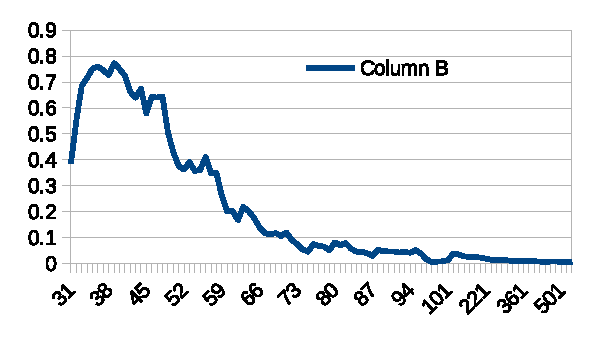
\includegraphics[width=8.4cm,height=3.5cm]{./Figures/avg-loss-donet.eps}
    \caption{Average loss}%
    \label{subfig:avg-loss-donet}
  \end{subfigure}
  \begin{subfigure}[c]{0.95\columnwidth}
    \centering
    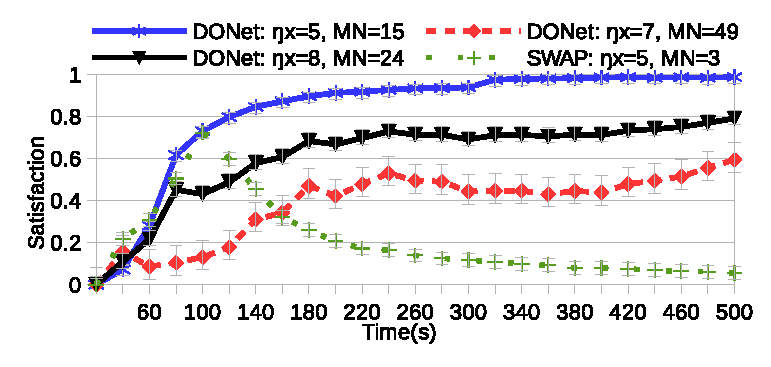
\includegraphics[width=8.4cm,height=3.5cm]{./Figures/satisfaction-donet.eps}
    \caption{Average peer satisfaction}%
    \label{subfig:satisfaction-donet}
  \end{subfigure}
  \caption{Attack's impact on DONet}%
  \label{fig:attack-results}
  \vspace{-4mm}
\end{figure}

% 
% 
% \begin{figure}[t!]
% \centering
% 
%   \mbox{\subfloat[Avg. loss]{\label{subfig:avg-loss-donet}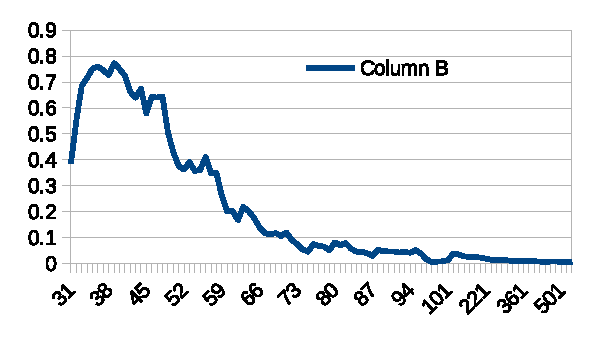
\includegraphics[width=8.4cm,height=3.5cm]{./Figures/avg-loss-donet.eps}}}
% %    \vspace{-3mm}
%   \mbox{\subfloat[Avg. peer satisfaction]{\label{subfig:satisfaction-donet}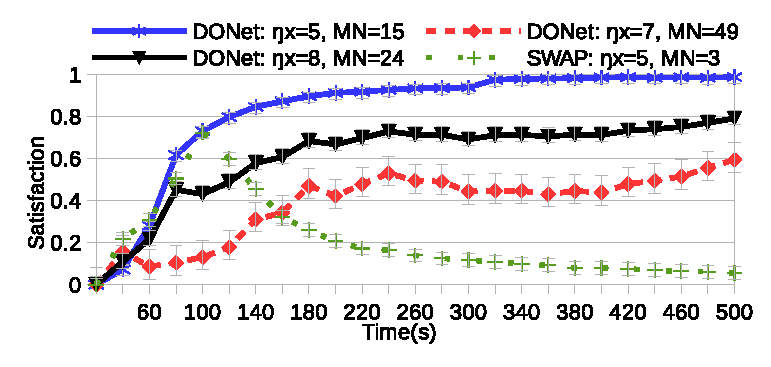
\includegraphics[width=8.4cm,height=3.5cm]{./Figures/satisfaction-donet.eps}}}
% %   \mbox{\subfloat[Avg. loss]{\label{subfig:avg-loss-donet}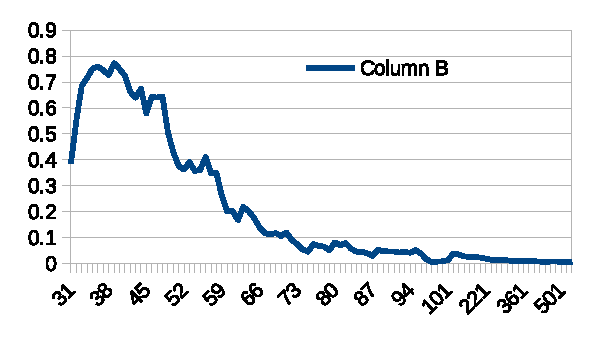
\includegraphics[width=3.7cm,height=2.5cm]{./Figures/avg-loss-donet.eps}} \subfloat[Avg. peer satisfaction]{\label{subfig:satisfaction-donet}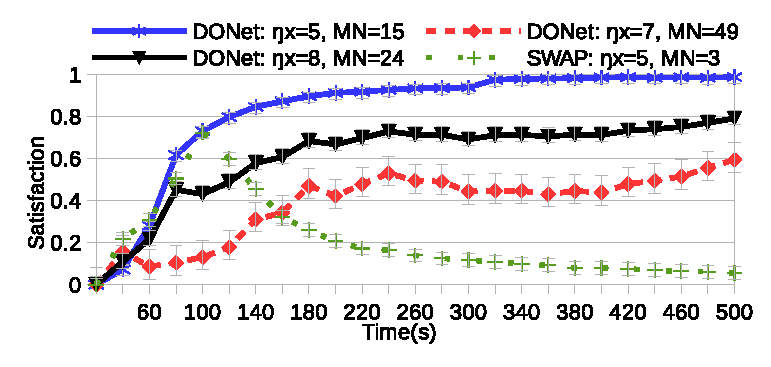
\includegraphics[width=3.7cm,height=2.5cm]{./Figures/satisfaction-donet.eps}}} 
% 
%   \caption{}
%   \vspace{-3.5mm}
%   \label{fig:attack-results}
%   \end{figure}
% 

\subsection{Case 2: Detection Mechanism Performance}

We now evaluate the performance of the detection mechanism.
Benign peers execute the detection mechanism as described in Section~\ref{sec:detection} whereas malicious peers aim to misuse the mechanism.
More precisely, malicious peers reply with a satisfaction level of 0 if the complaint might remove a benign peer and 1 if it might remove a malicious peer. 

In order to do so, we selected the following combinations for $(\eta x, MN)$: $(5, 80)$, $(8, 50)$ and $(10, 50)$ to assess the performance of the mechanism in severe attack conditions.
The satisfaction threshold $\satThres$ is set to 0.95 to measure if peers are able to fully restore their satisfaction level when the detection mechanism in operating.
The detection mechanism is effective starting $t=250s$ to allow for a reasonable amount of peers to join the overlay to adequately assess the efficiency of the mechanism.
In this scenario, every peer is allowed to initiate $\minDR=10$ detection requests for $t_{det}=500s$, and the minimum number of responses to generate a complaint is $\minP=3$. 
We discuss the effect of varying those parameters later on.

As depicted in Figure~\ref{subfig:BRNL}, once the detection mechanism is operating at $t=250s$, we observe an increase in the benign headnodes ratio in the source's neighbor list.
For instance, for $(\eta x, MN)=(5, 80)$, the source successfully attains ~80\% benign headnodes due to the detection mechanism.
For $(\eta x, MN)=(8, 50)$, the $BRNL$ ratio increases up to 90-100\%, which reflects the efficiency of the detection mechanism in replacing malicious headnodes to restore peers' satisfaction levels. 
Even if the source is initially only connected to malicious headnodes, i.e., $\eta x=10$, the detection mechanism is capable of restoring a $BRNL$ of close to 80\%. 

Figure~\ref{subfig:det-sat} illustrates the average restored peer satisfaction level due to the detection mechanism.
For the various attack placement strategies, the average satisfaction level increases up to ~95-100\%, even for $\eta x=10$.
As the detection mechanism starts at $t=250s$, the mechanism's impact on the peers' satisfaction level $\sat$ can be noticed in a short time period.
The reason is that the number of initial detection requests sent to the source results in replacing a high fraction of the source's headnodes and quickly increases the satisfaction levels. 
Moreover, malicious peers are unable to misuse the mechanism, as indicated by the absence of degradation in satisfaction levels. 

Figure~\ref{subfig:overhead} depicts the average detection overhead induced by our mechanism. 
As notice, the maximum overhead due to the detection mechanism is ~8\% for the different attack scenarios.
As peers are eventually satisfied, i.e., the number of detection requests initiated decreases, the overhead decreases to ~4\% at $t=500s$.
This implies that the overhead is not constant throughout time, i.e., once all peers' satisfaction level exceeds $\satThres$, they do not invoke the detection mechanism and hence do not induce additional overhead. 
Moreover, the maximum number of detection requests that can be initiated is dependent on $\minDR$, which is set to 10 in this scenario.
Thus, smaller values of $\minDR$ result in lower overhead, which is a useful application parameter that can be set according to suit the application's criticality or user's CPU resources.
In fact, varying $\minP$ between 3, 4 and 5 has little impact on the detection performance, indicating that nodes receive sufficient replies.

To that end, through the results, we highlight that the detection mechanism is indeed effective against \drop attacks, even if the attacker possesses high malicious budget as headnodes.
Moreover, we show that malicious peers are incapable of abusing the detection mechanism and place themselves as headnodes. Finally, the detection mechanism induces a very small overhead on the overlay.

\begin{figure}[tb]
%   \setlength{\belowcaptionskip}{-10pt}
  \centering
  \begin{subfigure}[c]{0.95\columnwidth}
    \centering
    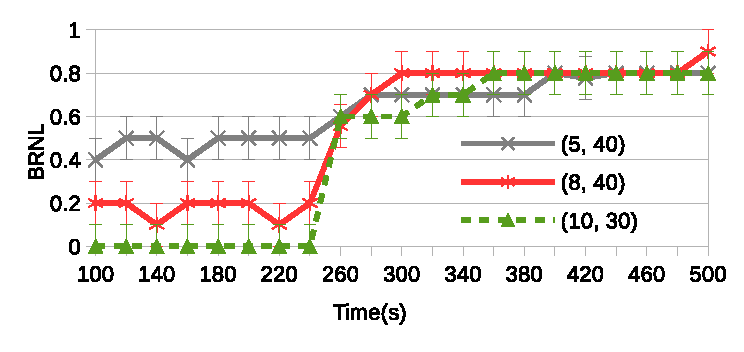
\includegraphics[width=8.4cm,height=3.5cm]{./Figures/det-BRNL1.eps}
    \caption{Average BRNL}%
    \label{subfig:BRNL}
  \end{subfigure}
  \begin{subfigure}[c]{0.95\columnwidth}
    \centering
    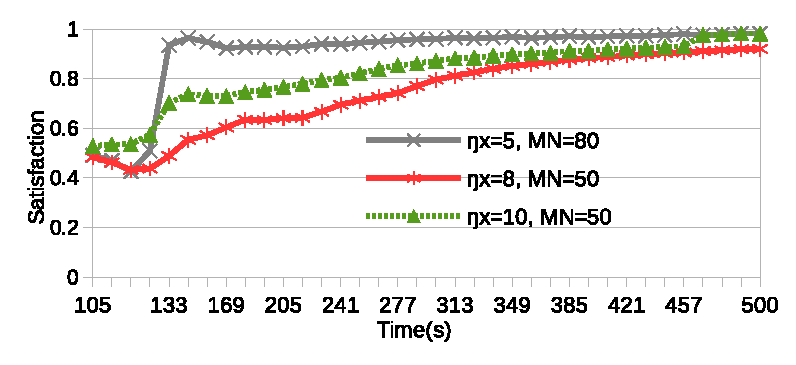
\includegraphics[width=8.4cm,height=3.5cm]{./Figures/det-sat.eps}
    \caption{Avg. peer satisfaction}%
    \label{subfig:det-sat}
  \end{subfigure}
  \begin{subfigure}[c]{0.95\columnwidth}
    \centering
    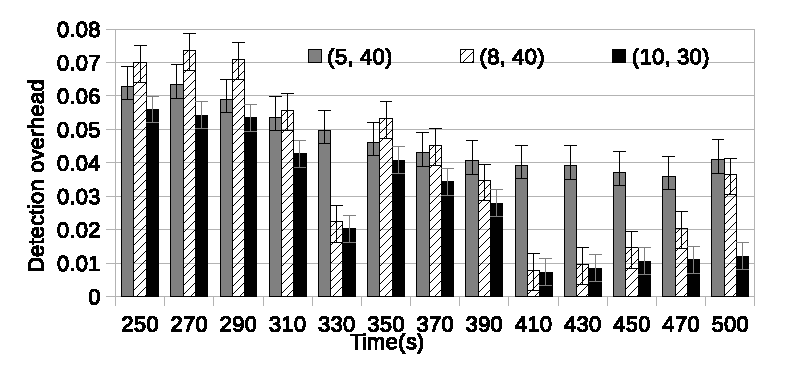
\includegraphics[width=8.4cm,height=3.5cm]{./Figures/overhead.eps}
    \caption{Detection overhead}%
    \label{subfig:overhead}
  \end{subfigure}
  \caption{Detection mechanism performance}%
  \label{fig:detection-results}
   \vspace{-4.5mm}
\end{figure}


% \begin{figure}[t!]
% \centering
% \vspace{-3.5mm}
%   \mbox{\subfloat[Avg. BRNL]{\label{subfig:BRNL}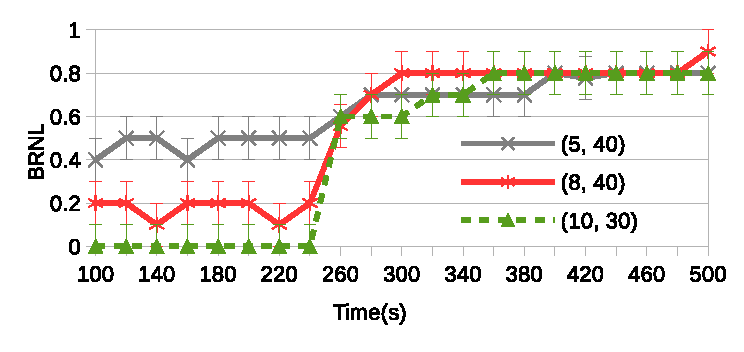
\includegraphics[width=8.4cm,height=3.5cm]{./Figures/det-BRNL1.eps}}}
% \vspace{-3.5mm}
%   \mbox{\subfloat[Avg. peer satisfaction]{\label{subfig:det-sat}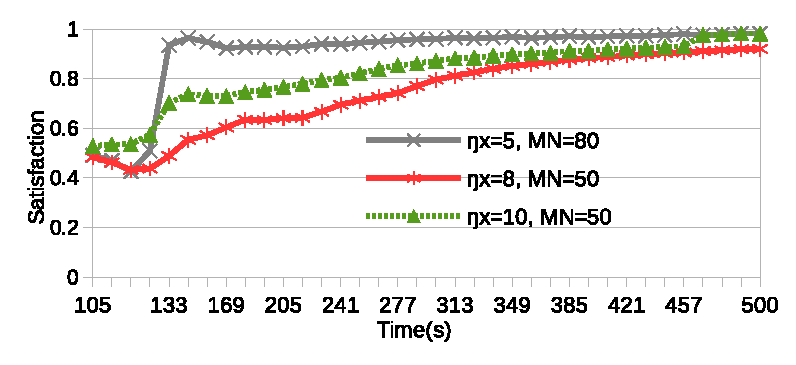
\includegraphics[width=8.4cm,height=3.5cm]{./Figures/det-sat.eps}}}
% 
%    \mbox{\subfloat[Detection overhead]{\label{subfig:overhead}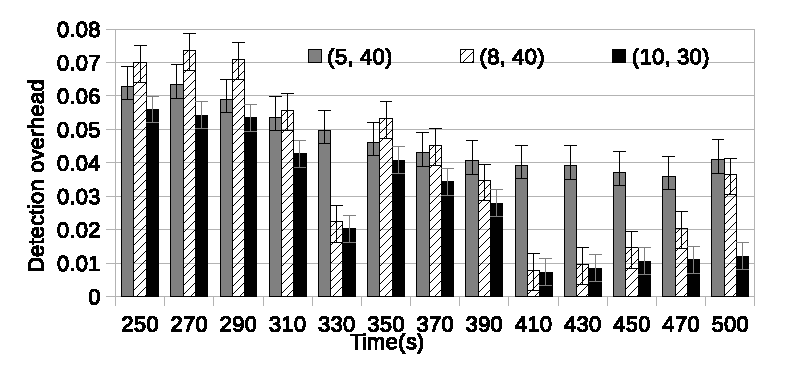
\includegraphics[width=8.4cm,height=3.5cm]{./Figures/overhead.eps}}}
% %   \vspace{-1.5mm}   
% %   \mbox{\subfloat[Avg. loss]{\label{subfig:avg-loss-donet}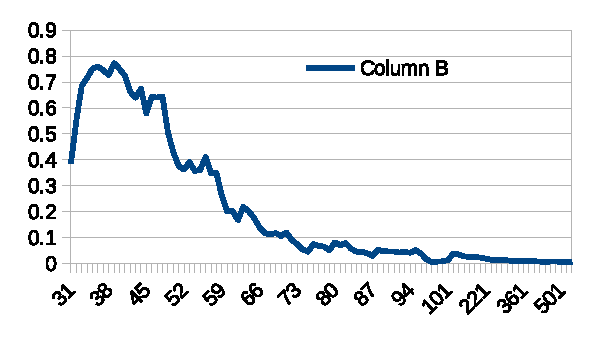
\includegraphics[width=3.7cm,height=2.5cm]{./Figures/avg-loss-donet.eps}} \subfloat[Avg. peer satisfaction]{\label{subfig:satisfaction-donet}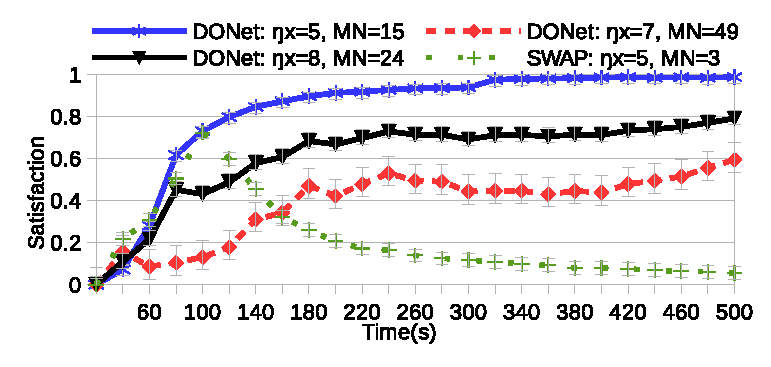
\includegraphics[width=3.7cm,height=2.5cm]{./Figures/satisfaction-donet.eps}}} 
% 
%   \caption{Detection mechanism performance}
%   \vspace{-3.5mm}   
%   \label{fig:detection-results}
%   \end{figure}


% \subsubsection{Summary of the results}
% 
% As a summary, for DONet, when the source's neighbor list is fully saturated with malicious peers, $IL$ is at ~100\%.
% Nevertheless, for smaller values of $Hx$, the attack's impact is still significantly high for a long period of time given the intolerability of such networks to such high delays.
% In fact, having only $Hx=\alpha$ without using $MN$ is sufficient for the attacker to completely isolate and thus, prevent the source from delivering any stream chunks.
% 
% For the SWAP case study, it is noticed that even with low values of $Hx$, after a certain swapping period, malicious peers manage to fully occupy the source's list and hence, $IL$ eventually reaches to ~100\%.
% This denotes that, the number of neighbors $MN$ is a major factor in the case of SWAP.
% Moreover, through an efficient distribution of the attacker's budget $x$, i.e., $Hx$ and $MN$, the attacker can decide whether to cause higher damage to the stream at the initialization time and then allow the network to eventually recover later on, or to allow the stream to reach to benign peers at earlier time phase till totally cutting the flow once $Hx=\alpha$ at some point.
\section{Detection \& Eviction}
\label{sec:detection}

In this section, we describe the main building blocks that constitutes proposed detection mechanism that targets detecting malicious peers in order to restore benign peers satisfaction.
We start by highlighting the general overview on how the detection mechanism flows.
Then, we describe the main differences between detecting a dropping attack behavior and detecting a manipulation/outdated chunks attack behavior, referred to as \textit{drop} attack, \textit{manp} attack for simplicity.
Afterwards, each detection sub-block, as illustrated in Figure~\ref{detection-blocks}, is presented.
The list of variables used throughout the paper is provided in Table \ref{tab:acronyms}.

\begin{table}[ht]
\center
\caption{Acronyms}
\begin{tabular}{|c|l||c|l|}
\hline

\bf{Var.} & \bf{Description}  & \bf{Var.} & \bf{Description} \\\hline\hline
$x$ & no. of malicious peers & $\eta$ & mal. headnodes fraction\\\hline
$MN$ & malicious neighbors & $\sigma$ & satisfaction threshold\\\hline
$H_n$ & list of headnodes & $P_n$ & potential candidates list \\\hline
$\alpha$ & manipulation threshold& $F$ & familiarity of suspect \\\hline
$G$ & suspect guilt value & $\kappa$ & dropping det. allowed\\\hline
$NL$ & neighbor list & $BM$ & buffer map\\\hline
\end{tabular}
\label{tab:acronyms}
\end{table}

\subsection{Mechanism Overview}
Here we describe an overall view for the flow of the detection mechanism before every process is detailed through the rest of the section.
Once a detection condition is triggered by a peer $b$, it sends a detection request to all peers that exist in its neighbor list.
Afterwards, for each peer who receives a request, prepares a reply according to the request ID, i.e., a \textit{drop} or a \textit{manp} request.
Once $b$ collects all the replies, it decides according to the proposed detection from the  in the replies to whether to fire a complaint to the source or not.
$b$ sends the complaint on behalf of the participating peers in the detection request. 
Finally, if $b$ sends a complaint to the source, the source decides about its content and replies back to $b$. In turn, $b$ forwards the source reply to the other participants in the complaint.

\subsection{Drop vs. Manp Detection}

On one hand, when $m$ conducts a drop attack on $b$, $b$ is not capable of detecting any malicious behavior.
Specifically, in a drop attack, $m$ never sends the actual $BM$ that represents the chunks it currently possesses, i.e., $m$ is only requesting chunks it already has.

On the other hand, in a manipulation or outdated chunks behavior, $m$ is eventually suspected as malicious since $b$ already expects the requested chunk from $m$.
Note that a peer might be overloaded due to a tight upload bandwidth or serving a lot of peers and thus, not able to serve all the requests.
Accordingly, the detection mechanism should differentiate between a malicious manipulating peer and an overloaded peer, which is discussed in Section~\ref{Detection-Trigger}.
To that end, through the rest of the section, we describe how the detection mechanism handles both cases: Drop and Manp detection.

\begin{figure}
 \centering
 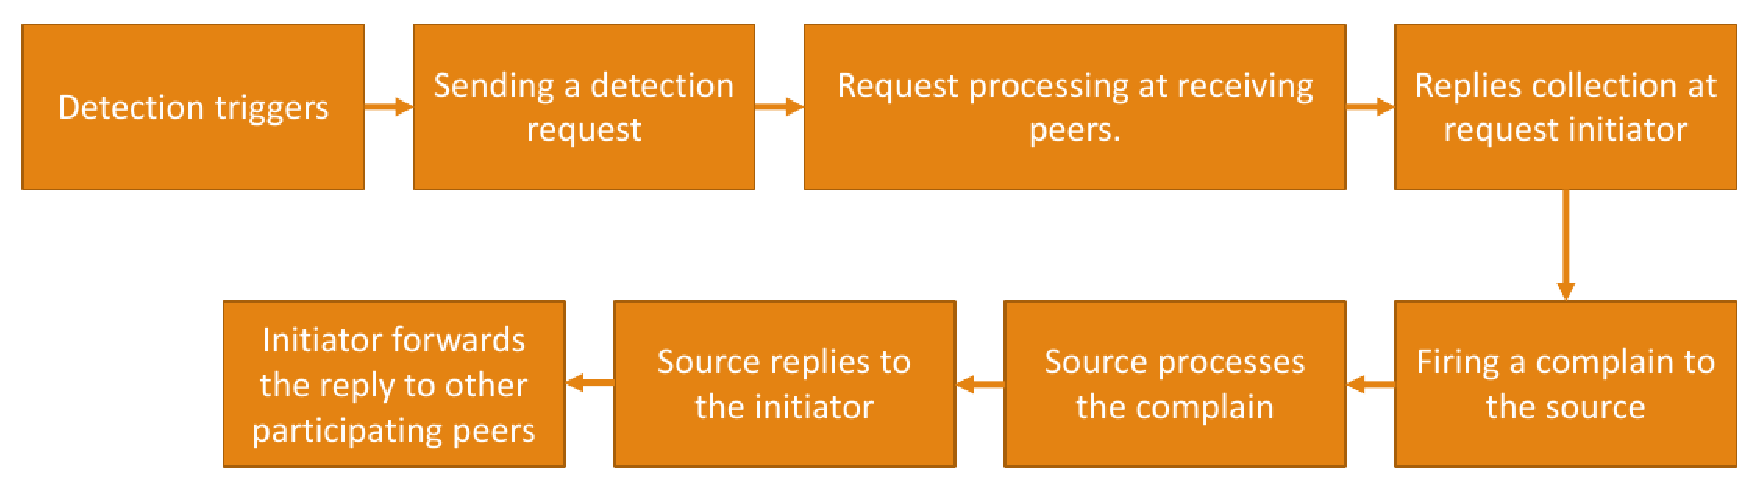
\includegraphics[width=8cm,height=3cm]{./Figures/detection-blocks.eps}
  \caption{Detection mechanism main blocks}
\label{detection-blocks} 
\end{figure}

\subsection{Detection Trigger}
\label{Detection-Trigger}
Here we describe how a peer decides on sending a detection request for both attack behaviors.
In both cases, once $b$ decides on sending a detection request, it only send it to peers in its own neighbor list $NL$ to check if those neighbors agree with it or not, disregarding the source if $b$ is a headnode.

Afterwards, as detailed in Section~\ref{Firing_a_Complain}, once $b$ receives its neighbors replies to the detection request, $b$ decides whether or not to fire a complaint to the source.
We assume that the source's address is publicly known and any peer can send a complaint to the source directly whether the source is already a neighbor to this peer or not.
\subsubsection*{Drop trigger}
In this, as there is no evidence of a manipulation from any neighbor to $b$, the only factor that $b$ is concerned about is the satisfaction threshold $\sigma$.
The satisfaction of a peer is defined as the fraction of missed chunks, i.e., the continuity of the stream according to the $Hit/Hit+miss$ chunk ratio.
In details, $b$ decides to trigger a detection request only if:
\begin{enumerate}
 \item $b$'s instant $satisfaction level < \sigma$.
 \item Number of drop detections sent by $b$ in the last $1000s$ is $< \kappa$.
\end{enumerate}
The latter condition guarantees that any peer can not trigger multiple detection requests in parallel so that: (a) to avoid exhausting the source's bandwidth, and (b) the source is most likely processing another peer's dropping request that might eventually positively impact $b$'s satisfaction level.
Note that in a drop attack, the detection request sent to $b$'s neighbors does not contain a certain suspect, hence, peers receiving a suspect-less request are aware that indeed it is a drop attack request.

\subsubsection*{Manp trigger}
$b$ decides to send a detection request if it was manipulated $\alpha$ times by $m$.
This condition essentially guarantees that any peer is not suspected instantly if it did not deliver the requested chunk, i.e., a benign peer might not deliver a chunk to the requester if it is already loaded serving other peers.
Obviously, $b$ attaches the suspect ID in the detection request to its neighbors.

In order to avoid malicious peers from abusing the manipulation detection mechanism, $b$ informs $m$ when $\alpha_m = \alpha -1$.
Accordingly, $m$ should give highest priority to $b$ and send the requested chunk signed and waits for a signed \textit{Ack} from $b$ as an evidence for not manipulating.
This evidence is later needed for the source to decide about $m$, as discussed in Section~\ref{Firing_a_Complain}.

\subsection{Processing Detection Request}
Here we describe how a peer $s \in S_b$, where $S_b$ is the set of peers who received a detection request from $b$ prepares a detection reply.
Note that as malicious peers the replies differ according to whether $s$ is malicious or benign, thus, we distinguish those two cases below. We refer to a malicious recipient as $s_m$ and a benign one as $s_b$.

\subsubsection*{Benign recipient}
Once $s_b$ receives a \textit{drop} request, it replies with its current satisfaction level as there is no exact suspect to give a detailed opinion about.
In case the request is a \textit{manp}, $s_b$ generates a reply the following three factors:
\begin{enumerate}
 \item \textit{familiarity $F$}: if $s_b$ is familiar with the suspect or not, i.e., is the suspect a current or a former neighbor of $s_b$ or not.
 \item \textit{Guilt $G$}: number of manipulation evidences $s_b$ has against the suspect. Note that this number is always $<\alpha$, otherwise, $s_b$ triggers a detection request on its own.
 \item \textit{Satisfaction}: the current satisfaction level of $s_b$.
\end{enumerate}


\subsubsection*{Malicious recipient}
Clearly, a malicious peer colludes with other malicious peers in the overlay. 
This means that $m$ always aim at providing the highest values that decreases the probability that $b$ reaches a decision to fire a complaint to the source, as detailed in Section~\ref{Firing_a_Complain}.
Hence, $s_m$ constantly tries to convince the detection initiator $b$ that it is fully satisfied in a \textit{drop} request, i.e., $satisfaction =1$.
In a \textit{manp} request, $s_b$ replies with $F=true, G=0, satisfaction=1$ in case the suspect is a colluding malicious peer.
Next, we describe how $b$ processes the values provided in the detection replies in order to reach a decision about firing a complaint to the source.

\subsection{Firing a Complaint}
\label{Firing_a_Complain}
Here we discuss the procedure applied by $b$ once it receives all detection replies for a certain request, or a waiting time-out $t_d$ occurs.
\subsubsection*{Drop request}
As discussed earlier, the only factor that $b$ can consider is $satisfaction$.
Thus, $b$ uses the following formula in order to decide about generating a complaint to the source:

\begin{align}
\label{eq:drop_satis_equation}
\sum_{i=0}^{z} satisfaction_i/z < \sigma
\end{align}
where $z$ is the total number of the received replies. 
In other words, $b$ sends a complaint only if the average satisfaction level of its neighbors is below than the predefined satisfaction threshold $\sigma$.

To prevent malicious peers from abusing the drop detection mechanism and cause an illusion at the source that a general dissatisfaction is detected, the following conditions are applied:
\begin{enumerate}
 \item Each peer can at most generate or participate in maximum $\kappa$ drop complaints to the source per $1000s$.
 \item No simultaneous generation or participation in more than one complaint is allowed to any peer, i.e., once a node is engaged in a detection process, it should wait till the final decision is reached.
\end{enumerate}
Those conditions guarantee that malicious peers indeed can not abuse the drop detection mechanism, however, benign peers as well have the same constraints which might reside in a benign peer not able to eventually complain to the source.
For those reasons, as we further elaborate on Section~\ref{complaint_source}, once a drop detection complaint reaches the source, the fraction of headnodes replaced is large in order to maximize the likelihood of affecting a large fraction of peers, specially for peers who might not be able to complain to the source at the moment.

\subsubsection*{Manp request}
In this simpler case where a certain suspect already exists, $b$ decides to fire a complaint if the following conditions hold:

\begin{align}
\label{eq:drop_familiarity_equation}
\sum_{i=0}^{z} F_i > z/2
\end{align}
The condition in \ref{eq:drop_familiarity_equation} guarantees that at least more than half of the participant peers have information about the suspect, i.e., the suspect is an entry in their neighbor list.
Note that for any peer, $F_i = 0 | 1$.

Next, for peers who are \textit{familiar} with the suspect, the total average \textit{Guilt} must be greater than the maximum amount of \textit{Guilt} that can be reported by familiar peers, as stated in ~\ref{eq:drop_guilt_equation}.

\begin{align}
\label{eq:drop_guilt_equation}
\sum_{i=0}^{z} G_i > \sum_{i=0}^{z} F_i*(\alpha-1)/2
\end{align}
Nevertheless, the same condition for dropping attack in \ref{eq:drop_guilt_equation} is also considered in a \textit{Manp}.
Thus, we assure that the participating peers are currently unsatisfied, i.e., peers might have $m$ in their suspect list $G$ but still they are satisfied through other peers and no gain for them from firing a complaint.


\subsubsection*{Firing a complaint to the source}

Once $b$ decides on firing a complaint according to the aforementioned criterion, $b$ generates a complaint message to the source.
In a \textit{Manp} scenario, $b$ attaches the following information to the complaint message: (a) IDs of \textit{familiar} peers, (b) evidences of manipulation gathered from the replies, (c) per reply values of $G,satisfaction$ and (d) suspect ID.
While in a \textit{Drop} scenario: (a) IDs of all participating peers, and (b) $satisfaction$ value in each reply.

\subsection{Processing a Complaint at the Source}
\label{complaint_source}
At this point the source receives a complaint from $b$, the source decides on the next procedure depending on whether the complaint is a \textit{Drop} or a \textit{Manp}.
Note that the source can identify the request's type based on the suspect field, i.e., in case of no suspect attached, it is indeed a \textit{Drop} complaint.

\subsubsection*{Manp request}
We start with the simpler case of receiving a \textit{Manp} request, where the source executes the following steps:
\begin{enumerate}
 \item Checks the validity of all manipulation attached, as discussed in Section~\ref{Detection-Trigger}.
 \item If the above checked is passed, the source removes the suspect from its neighbor list.
 \item Saves the free entry in its list after removing the suspect for $b$ to connect and be a headnode. Hence, all peers participating in the complaint will be directly connected to a headnode which remarkably enhance their satisfaction level.
 \item The suspect is added to a blacklist, i.e., the suspect is not allowed to be a headnode again.
 \item Generating a \textit{Complaint Reply} to $b$ confirming blacklisting $m$.
\end{enumerate}

\subsubsection*{Drop request}
Now we consider the \textit{Drop} complaint. The source conducts the following procedure:
\begin{enumerate}
 \item Divides the set of participating peers into two sets $H_n$ and $P_n$.
 $H_n$ contains peers in the complaint that are already headnodes.
 \item Removes all peers in $H_n$ from its neighbor set.
 \item Randomly connects to other peers. The reason behind not connecting to a fraction of the participating peers in the complaint is to avoid the probability that malicious peers are abusing the detection mechanism in order to get connected as headnodes.
 \item Adds peers (excluding peers in $H_n$) from its neighbor list to $P_n$, where $P_n = neighborList\setminus H_n$.
 \item Sends a \textit{Complaint Reply} to $b$ containing $H_n$ and $P_n$.
\end{enumerate}

\subsection{Processing a Complaint Reply \& Forwarding}

As the last procedure, when $b$ receives the \textit{complaint Reply} from the source, $b$ performs the following procedure, which again differs based on the complaint type (\textit{Drop} or \textit{Manp}).
In a \textit{Manp} scenario, $b$ executes the following procedure:
\begin{enumerate}
 \item Disconnects and blacklist the suspect.
 \item Connects to the source, if for abnormal reasons the connection is not possible, $b$ connects to a random peer.
 \item Forwards the \textit{Complaint Reply} to all peers who agree about $m$ being malicious, i.e., familiar peers with $G > 0$.
\end{enumerate}
Finally, the participating peers performs step 1 and 2 once they receive the forwarded reply.

For a \textit{Drop} scenario, $b$ follows the next procedure:
\begin{enumerate}
 \item Disconnects from all peers in $H_n$. Note that peers in $H_n$ are not expelled from $b$'s neighbor list due to the fact that those peers are not proven malicious.
 \item Connects to $|H_n|$ peers from $P_n$, in case $|H_n|>|P_n|$, peers connect to $|P_n|+(|H_n|-|P_n|)random peers$.
\end{enumerate}
Similarly, $b$ forwards the complaint to the other participants who in turn executes steps 1 and 2.

\subsection{General Notes}
The detection mechanism does not aim at expelling peers from the system.
The reason behind that is the \textit{Drop} adversarial behavior, where basically benign peers are equally probable to be removed from the source's neighbor list as malicious ones.
Thus, the impact on such peers is minimized, i.e., they are not entirely expelled from the system or even from the peers participating in the complaint neighbor list.
In general, the main target of the detection mechanism in a \textit{Drop} case is to enhance the peers satisfaction level while minimizing: (a) peers replacements, (b) detection overhead, and (c) malicious peers chances to abuse the detection mechanism.

Unlike in a \textit{Drop} detection complaint, peers proved malicious through out the detection process are placed at relatively distant positions from the source.
Hence, such peers impact on delivering chunks to other peers is less critical than peers at headnodes or neighboring headnodes.
In the following section, we evaluate our mechanism's performance and accuracy, along with demonstrating the attack's severity.





\section{Analysis}
\label{sec:analysis}



%Due to the high flexibility of pull-based content distribution and the corresponding loose correlation between a node's position in the network and its satisfaction, 
We focus on characterizing the behavior of malicious nodes aiming to subvert the detection mechanism to remove honest headnodes and retain malicious ones. 
%Hatem: trim
% More precisely, we show that successfully accusing a benign headnode of cheating requires that the malicious peer starting the complaint presents a neighbor list that is either dominated by malicious peers or contains benign peers with unusually low satisfaction levels.
More precisely, we show that successfully accusing a benign headnode of cheating requires that the malicious peer issuing a complaint presents a neighbor list that is either dominated by malicious peers or by benign peers with unusually low satisfaction levels.
Similarly, preventing the removal of a malicious headnode requires that a high number of the  neighbors are malicious.


%Recall that a \drop request issued by a node $u$ succeeds in removing a headnode $h$ if the average satisfaction level in the responses that $u$ sends to the source is below a threshold $\satThres$.  

\subsection{Falsely Accusing Benign Headnodes}

We start by considering the case that malicious nodes want to misuse the detection mechanism to remove a benign headnode. 
Note that there are reliable methods to identify headnodes~\cite{nguyen2016swap}, so malicious peers are likely to know if one of their neighbors is a headnode.  
The malicious node $m$ initiating a request with the goal of removing one benign headnode can manipulate the set $D$ of nodes whose satisfaction levels $m$ forwards to the source. 
In other words, after querying all nodes in its actual neighbor list, $m$ might send only  subset of the responses as well as responses from additional nodes to the source. If possible, $m$ chooses these responses in such a manner that the source will remove the benign headnode. 
There are restrictions guiding the construction of $D$ that $m$ has to take into consideration:
\begin{itemize}
%Hatem: trim
% \item $m$ has to include the benign headnode that it aims to remove. 
\item $m$ should include the benign headnode it aims to remove. 
% \item $m$ cannot include benign nodes that are not in its actual neighbor list, as $m$ does not have valid proofs of neighborhood. 
\item $m$ cannot include benign nodes that are not in its actual neighbor list, as $m$ has no valid proofs of neighborhood. 
\item $m$ does not have to include all peers that are in its actual neighbor list, as there is no possibility to detect excluded neighbors short of asking all peers in the system if they are neighbors of $m$. 
\item $m$ can include malicious peers that are not in its actual neighbor list, as these peers are willing to generate false proofs of neighborhood. Only the inclusion of malicious nodes that can participate in a \drop request, i.e., those that have not yet reached their limit of \drop request participation, is beneficial for the success of the request. Malicious peers contained in $D$ claim that their satisfaction level is 0 to maximize the chance of removal. 
\end{itemize}

When deciding on a set $D$, $m$ tries to minimize the number of malicious nodes in $D$ in order to use as little of the attack budget as possible. 
Preposition \ref{prop:dropping-removal} states the number of malicious nodes that have to be involved for the request to succeed and the proof illustrates the strategy for choosing the set $D$. 
Preposition \ref{prop:dropping-removal} states the number of malicious nodes that have to be involved for a successful request and the proof illustrates the strategy for choosing the set $D$. 

For simplicity, Preposition~\ref{prop:dropping-removal} considers the case that only one headnode is contained in $m$'s neighbor list. In the presence of several headnodes, $m$ has to slightly adapt its attack strategy. 
If additional malicious headnodes are neighbors of $m$, $m$ does not include the respective nodes in $D$ to avoid accidentally causing the removal of malicious headnodes.  In contrast, if additional benign headnodes are neighbors of $m$, $m$ will include all of them in $D$ if the detection request can be successful. If success is not possible due to the high satisfaction level of the included headnodes, $m$ successively removes each headnode using the strategy outlined in Preposition~\ref{prop:dropping-removal}.   
 

\begin{proposition}
\label{prop:dropping-removal}
Let $m$ be a malicious neighbor of a benign headnode $h$ with satisfaction level $\sat_h$. Assume that $m$ has $k$ benign neighbors $v_1, \ldots , v_k$ sorted by their satisfaction levels $\sat_1 \leq \sat_2 \leq \ldots  \leq \sat_k$. 
%Hatem:edited this line with: to successfully remove $h$
Then, to successfully remove $h$, $m$ has to include at least $c$ responses of malicious nodes, including $m$ itself, in the set $D$ of forwarded responses such that:
\begin{align}
\label{eq:drop-rem}
\begin{split}
c &= \max \Big( 1,  \\
 & argmin_{c' in \mathbb{N}} 
\left\lbrace \frac{1}{\minP}\left(\sat_h+\sum_{i=1}^{\minP-c'-1}\sat_i \right) < \satThres \right\rbrace 
\Big)
\end{split}
\end{align}
%Hatem: trim (this line was added above)
% to achieve the removal of $h$. 
\end{proposition}
\begin{proof}
To remove the headnode $h$, there has to be a detection requests containing the responses of $h$ and $n\geq \minP-1$ nodes with satisfaction levels $s_1, \ldots , s_n$ and 
$\frac{1}{n+1}\left( s_h + \sum_{i=1}^{n}s_i \right) < \satThres$.
The node $m$ aims to minimize the number of involved malicious nodes $c$ because each malicious node can only participate in $\kappa$ detection requests per interval. At the same time, $m$ has to ensure that the average satisfaction level of the involved nodes is below $\satThres$ and that the request includes at least $\minP$ nodes in total. As $m$ files the request, at least one malicious node has to be included. 
In other words, $m$ solves the optimization problem of finding a minimal $c$ and a set of integers $I \subset \{1, \ldots, k\}$ such that i) $c + |I|+1 \geq \minP$, ii) $\frac{1}{c + |I|+1}\left( \sat_h + \sum_{i \in I} sat_i \right) < \satThres$, and iii) $c\geq 1$. 
Choosing the lowest satisfaction levels indeed solves the optimization problem and results in Eq.~\ref{eq:drop-rem}. 
\end{proof}

Proposition~\ref{prop:dropping-removal} indicates that a high number of malicious peers have to participate in the removal of one honest headnode if the satisfaction levels are high. 
For instance, if all benign peers have a satisfaction level of 1, then Eq.~\ref{eq:drop-rem} states that $\lfloor \satThres*t \rfloor +1$ malicious peers are required to remove \emph{one} benign headnode.
As the source chooses the replacement headnode randomly, the new headnode is likely benign. 
Hence, under the assumption of a low attacker budget, the attacker might only be able to remove 1-2 headnodes per interval and does not manage to place its own nodes as headnodes. 

\subsection{Retaining Malicious Headnodes}
Now, we consider the case that malicious nodes collude to retain one or several malicious headnode when a benign peer initiates a detection request that includes these malicious headnode in the neighbor list. 
All malicious nodes in the respective neighbor list will provide a satisfaction level of 1 to prevent the removal of a malicious node. We assume that malicious neighbors will try to prevent the removal of malicious headnodes even if the request can in addition result in the removal of benign headnodes. This assumption seems reasonable as the removal of a benign headnode is unlikely to lead to an additional malicious headnodes, indicating that retaining existing malicious headnodes is of higher importance than removing benign headnodes.  Preposition~\ref{prop:dropping-retain} provides the condition governing the success or failure of the \drop request in the face of the proposed adversarial behavior. 

\begin{proposition}
\label{prop:dropping-retain}
Let $m$ be a malicious headnode and $b$ be a benign neighbor of $m$ that initiates a detection request due to its low satisfaction level $\sat_b$.
Assume that $b$ has $k$ benign neighbors $v_1, \ldots , v_k$ with satisfaction levels $\sat_1, \sat_2 ,\ldots  , \sat_k$. In addition, $b$ has $y$ malicious neighbors, which includes the malicious headnode, and $k\geq \minP$.
 Then the removal of $m$ fails if and only if: 
\begin{align}
\label{eq:drop-retain}
\frac{1}{k+y+1}\left(y+\sat_b + \sum_{i=1}^k \sat_i\right) \geq \satThres.  
\end{align} 
\end{proposition}
\begin{proof}
The claim follows directly as all $y$ malicious peers will set their satisfaction level to 1 and \drop requests with an average satisfaction of at least $\satThres$ are not successful.   
\end{proof}
If the condition $k\geq \minP$ in Preposition~\ref{prop:dropping-retain} does not hold, the malicious nodes have the option of undermining the request by not responding. 
However, the attacker generally does not know the number of benign neighbors and hence cannot strategically decide whether to answer. 
Refusing to answer if actually $k\geq \minP$ is likely to lead to the removal of the malicious peer as the malicious peers forfeit their opportunity to influence the average satisfaction level. 
Thus, we assume that malicious peers indeed always reply with a satisfaction level of 1. 

Proposition~\ref{prop:dropping-retain} indicates a successful removal of malicious nodes unless the satisfaction level of benign peers remains high or the neighborhood of the benign peer contains many malicious peers. 
If indeed satisfaction levels remain high, then no real need to remove the malicious peer.
In contrast, it is highly unlikely that an honest peer is surrounded by malicious peers if the attack budget is low.
Even if one neighbor of the malicious headnode has primarily malicious neighbors, other benign neighbors are likely to file a complaint.
Dominating the neighborhood of all of $m$'s neighbors should not be possible for the attacker due to its limited resources.

 
 
\section{Related Work}
\label{sec:related}

We overview the prominent existing work on attacks and attack detection in the area of P2P streaming systems. Most prior work has considered three attack types: (i) pollution attacks, i.e., flooding the overlay with arbitrary content and claiming it to be relevant chunks, (ii) free riding, i.e., participating in the overlay without contributing, and iii) cheating attacks, i.e., maliciously dropping packets or manipulating buffer-maps. 

Pollution attacks are one of the most common attacks \cite{pollution1}. 
As the attack strategy differs from the \drop attack and efficient network coding techniques \cite{nc} and others \cite{pollution2} already exist, we do not consider those attacks in our work.
% Consequently, researchers have studied them extensively and there exist various detection and mitigation schemes .    
% As the existing approaches seem to render the attack harmless, we do not focus on it in this work but rather assume that appropriate measures against these attacks such as network coding  are already in place.

In contrast, the main approach to counter free riding are incentives \cite{defending,defending2}, i.e., rewarding peers that distributed the stream to others; 
% e.g., with an increased flexibility in the neighbor selection or positions closer to the source to receive a better service. 
% As a consequence, free riders likely end up far from the source, meaning that they are not required to forward the stream anyways, because all their neighbors already requested the chunks from others by the time the free riders receive them. 
However, these strategies are only effective for peers that aim to minimize their level of participating. 

% Hatem: trim
% Cheating attacks are severe denial-of-service attacks, performed with the goal of maximizing the damage to the overlay and preventing peers from downloading the video.   
Cheating attacks are severe DoS attacks, performed to maximize the damage to the overlay and preventing peers from downloading the stream.   
\textit{Antiliar} is a general defense mechanism against a diverse set of attacks, including dropping and buffer map manipulation\cite{antiliar}.
Mainly, \textit{Antiliar} tracks peers behaviors in a secure progress log and thus, detecting misbehaving peers by identifying irregularities in the log. 
While highly effective, \textit{Antiliar} relies on expensive cryptographic operations that are unsuitable for devices with low CPU resources.
Moreover, \textit{Antiliar} uses a central entity to review the logs, creating additional security and privacy problems. 

An alternative approach \cite{nguyen2014resilience} relies on redundancy by enforcing diversity when requesting chunks. 
In this manner, the attacker has to control a higher fraction of nodes to achieve any severe damage by cheating.
The work focuses in particular on attacks on headnodes yet assumes an external attacker that can take over arbitrary nodes at will.
In this context, the idea of swapping headnodes frequently to mitigate the impact of the attacker's control can significantly decrease the attack severity \cite{nguyen2016swap}.
As shown in Section~\ref{sec:eval}, internal attackers can undermine the swapping protocol and gain the position of headnodes.  

\section{Conclusion \& Future Work}
\label{sec:conclusion}


 \bibliographystyle{unsrt}
 \bibliography{ref}

\IEEEpeerreviewmaketitle


\end{document}
	